\textbf{مورد استفاده:}
داشبورد کارفرما
\\
\textbf{شرح مختصر :UC}
در این قسمت داشبورد کارفرما را در اختیار کاربر قرار می‌دهد.
\\
\textbf{پيش شرط:}
ورود به داشبورد کارفرما.
\\
\textbf{سناريو اصلی:}
\begin{enumerate}
	\item
	شروع
	\item
	کارفرما به بخش‌های مختلف مانند ایجاد و اصلاح پروژه، انتخاب فریلنسر برای پروژه و .. دسترسی پیدا می‌کند.
	\item
	پایان
\end{enumerate}

\noindent
\textbf{پس شرط:}
ندارد.
\\
\textbf{سناريوهای فرعی:}
ندارد.
\\
\textbf{پس شرط:}
ندارد.


\begin{figure}[H]
	\centering
	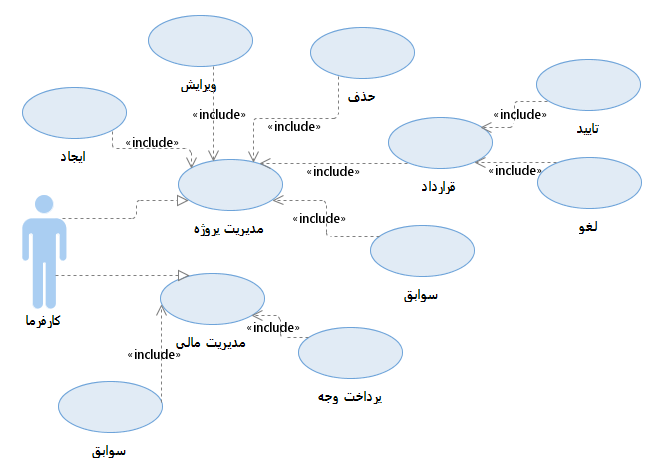
\includegraphics[width=.7\textwidth]{Diagram/1.UseCase/داشبورد-کارفرما.png}
	\caption{دیاگرام UC ‌داشبورد کارفرما}
	\label{fig:uc:داشبورد-کارفرما}
\end{figure}